\section{EELS analyses of TMDs nanostructures}
\label{sec:tmd}
\label{sec:eels}

In this work we apply our machine learning method to the study
of the low-loss EELS region for a specific type of WS$_2$ nanostructures known
as nanoflowers.
%
WS$_2$ is a transition metal dichalcogenide (TMD) material, which in turn
belongs to a class of materials known as two-dimensional, van der Waals, or simply layered materials.
%
These materials are
characterised by the remarkable property of being fully functional down to a single atomic layer.
%
In order to make the present study self-contained and accessible to a wider audience,
in this section we review the basic concepts underlying the EELS
method and discuss some of its recent applications to the study of TMDs nanostructures with emphasis
on WS$_2$.

\subsection{EELS in a nutshell}

Electron energy loss spectroscopy is a TEM-based method
whereby an electron-transparent sample is illuminated by a 
beam of energetic electrons.
%
Subsequently to the crossing of
the specimen, the scattered electron beam is focused by a magnetic prism
towards a spectrometer where the distribution of electron energy losses $\Delta E$ is recorded.
%
As schematic illustration of a typical EELS setup shown in the left panel of Fig.~\ref{fig:EELS}.
%
EEL spectra can be recorded either in the Scanning Transmission Electron Microscopy (STEM)
or in the conventional TEM modes.
%
Thanks to recent progress in TEM instrumentation and data acquisition, state-of-the-art EELS analyses befit from
a highly competitive energy (spectral) resolution combined with an unparalleled spatial resolution.

%%%%%%%%%%%%%%%%%%%%%%%%%%%%%%%%%%%%%%%%%%%%%%%
\begin{figure}[t]
    \centering
    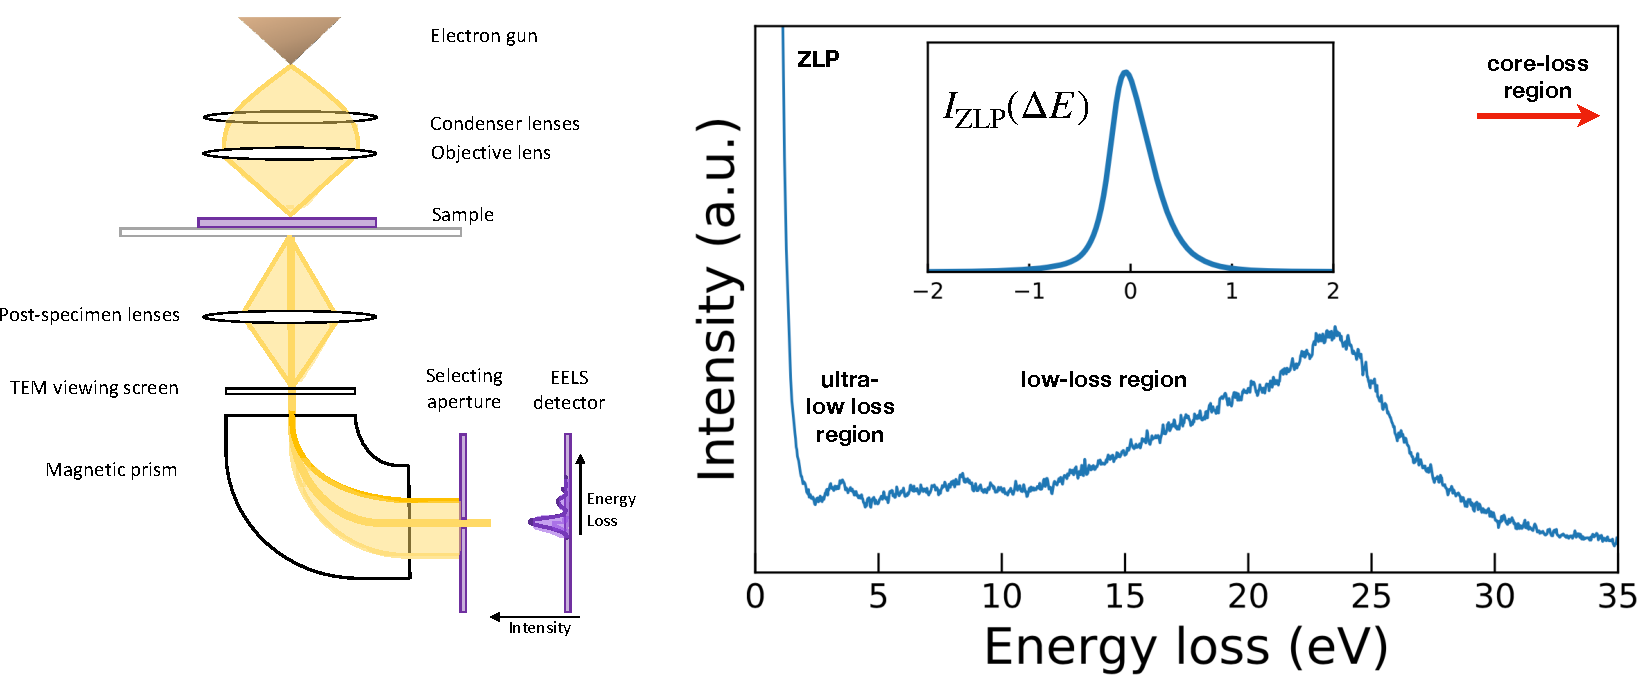
\includegraphics[width=0.9\textwidth]{plots/EELS.pdf}
    \caption{Left: in STEM-EELS, a magnetic
      prism is used to deflect the electron beam after crossing the sample
      so that the distribution of their energy losses $\Delta E$ can be recorded.
      %
      Right: a representative spectrum for $\Delta E \le 35$ eV acquired 
      on a WS$_2$ nanoflower~\cite{SabryaWS2} with
      the inset displaying the corresponding ZLP.
      }
    \label{fig:EELS}
\end{figure}
%%%%%%%%%%%%%%%%%%%%%%%%%%%%%%%%%%%%%%%%%%%%%%%%5

EELS spectra can be divided into three main regions.
%
The first one is the zero-loss region, centered around $\Delta E=0$
and that contains the contributions from both elastic scatterings
as well as those from electrons that have not interacted with the
sample.
%
This region is characterised by the strong, narrow ZLP which is there  much larger than the contribution
from inelastic scatterings.
%
The second region is the low-loss region, is characterised by energy losses
$\Delta E \lsim 50$ eV, and which contains information
about several important features of the studied sample such as plasmons, excitons, phonons, and
intra-band transitions.
%
Of particular relevance in this context is the ultra-low loss region, characterised by $\Delta E \simeq$ few eV
and where the contributions of the ZLP and that from the inelastic scatterings
off the sample are comparable.
%
For $\Delta E \gsim 50$ eV one then has the core-loss region,
which is provides compositional information
on the materials that constitute the sample.
 
The right panel of Fig.~\ref{fig:EELS} displays
a representative EELS spectrum in the region $\Delta E \le 35$ eV, recorded
on one of the WS$_2$ nanostructures presented~\cite{SabryaWS2}
and which will be further discussed in Sect.~\ref{sec:tmd}.
%
The inset displays the Zero Loss Peak, illustrating how
its magnitude is larger than the contribution from the inelastic scatterings
off the sample by several
orders of magnitude.
%
Clearly, carefully disentangling these two contributions in the region $\Delta E \simeq$ few eV
is essential for the physical interpretation of EEL spectra in the ultra-low-loss region.
%
The magnitude and shape of the ZLP intensity is known to depend not only on the specific values
of the electron energy loss $\Delta E$, but also in other operation parameters
of the TEM such as the electron beam energy $E_{\rm beam}$ and the exposure time
$T_{\rm exp}$, the aperture width and the use of a monochromator. 
%
This means that in general one cannot measure the ZLP for a given operation
conditions, say a high beam voltage of $E_{\rm b}=200$ keV, and expect to reproduce
the ZLP associated to different conditions, such as a  high beam voltage of $E_{\rm b}=60$ keV,
without introducing a specific model.
%
Several attempts to model the ZLP peak have had some success at fitting the main intensity of the peak, 
but in the tails discrepancies are as large as 25-35\%~\cite{Bangert:2003}.
%
The standard background 
subtraction method is to fit a power law to the tails, however this subtraction is not suitable in
many circumstances and regimes~\cite{Hachtel:2018, Tenailleau:1992, Reed:2002, Bosman:2006}.
%
Unfortunately, it is not possible to compute the dependence of the ZLP on $\Delta E$
and the rest of operation parameters of the microscope from first principles.
%
Further, even for identical operation conditions the value of the ZLP
will in general vary due to {\it e.g.} external perturbations such as electric or magnetic fields~\cite{Rafferty:2000},
the stability of the microscope and spectrometer electronics~\cite{Kothleitner:2003}, the local
environment (possibly exposed to mechanical vibrations and pressure and temperature fluctuations) 
and spectral aberrations\cite{Egerton:1996, Scherzer:1949}. 
%
Any model for the ZLP should thus account for this irreducible source of uncertainties.
%
In this work we will investigate EELS measurements collected  on a cold field emission gun JEOL
transmission electron microscope operating at different beam energies $E_{\rm beam}$
and equipped with a  Gatan spectrometer.
%
The energy resolution is of these measurements,
defined as the FWHM of the ZLP, is $\delta E=40$ meV.
%
These measurements have a spatial resolution of ...

%%%%%%%%%%%%%%%%%%%%%%%%%%%%%%%%%%%%%%%%%%%%%%%%%%%%%%%%%%
%%%%%%%%%%%%%%%%%%%%%%%%%%%%%%%%%%%%%%%%%%%%%%%%%%%%%%%%%%



Perhaps the most renowned member of this family of materials is graphene,
which benefits from many interesting properties such as efficient heat and electricity conduction.
%
However, under normal conditions graphene lacks of a band gap, hampering its potential
applications in nano-electronics.
%
Recently, significant attention has been devoted to other types
of two-dimensional materials known as  transition metal dichalcogenides (TMDs).
%
These materials are of the form MX$_2$, where M is a 
transition metal atom (such as Mo or W) and X a chalcogen atom (such as S, Se, or Te). 
%
The crystalline structure of TMDs is such that
one layer of M atoms is sandwiched between two layers of X atoms.

The electronic structure of TMDs strongly depends on the coordination 
of the transition metal atoms, giving rise to an array of electronic
and magnetic properties~\cite{Chhowalla:2013}.
%
Further, the properties of this class of materials vary quite significantly
with their thickness, for instance MoS$_2$ exhibits an indirect bandgap
in the bulk form while it becomes direct at the monolayer level~\cite{Splendiani:2010}.
%
Such a tunable electronic structure and the potential applications in
nano-electronics makes these materials highly attractive for research. 

In this work we are interested in studying of the local electronic
properties of tungsten disulfide, WS$_2$, specifically of the
WS$_2$ nanostructures presented in~\cite{SabryaWS2}.
%
This material also exhibits an indirect-to-direct bandgap transition when going
from bulk to bilayer or monolayer form.
%
The effects of this transition are manifested as enhanced
photoluminescence in monolayer WS$_2$, whereas only little emission is observed in
the corresponding bulk form.
%
Further applications of this material include storage of hydrogen 
and lithium~\cite{Bhandavat:2012} for batteries.

As for other TMD materials, WS$_2$ adopts a layered structure 
by stacking atomic layers of S-W-S in a sandwich-like configuration. 
%
Although the interaction between adjacent layers is a weak Van der Waals 
force, the dependence of the interlayer interaction on the stacking 
order of WS$_2$ is significant.
%
Therefore, modulating the electronic
structure in a well-controlled way is crucial for application to
nano devices.
%
As discussed in~\cite{SabryaWS2},
a phenomenon called polytypism is an important factor that determines the interlayer
interactions within WS$_2$: different stacking types tend to coexist, 
complicating the characterization of the physical properties~\cite{Na:2018}.
%
One response of different stacking patterns to electric fields is
spontaneous electrical polarization, leading to modifications on the 
electronic band structure and correspondingly on the band gap~\cite{Li:2016}.

In this work we will analyse EEL spectra taken on WS$_2$ flower-like nanostructures~\cite{SabryaWS2}.
%
These nanoflowers  exhibit a  variety of morphologies, including lying flakes (“petals”) and
edge-exposed standing petals, arising from a common point (the “stem”).
%
 Structural analysis reveals that they exhibit a mixture of the 2H and 3R crystalline phases. 
%
EELS measurements were used to reveal the nature of the surface and edge excitations in these WS2 nanoflowers.

One of the interesting properties of  WS$_2$ is
that when the material
thinned down to a single monolayer, its indirect band gap switches to a direct band gap of approximately 2 eV.
%
In general, it has been found that the type and magnitude of the bandgap
of WS$_2$ depends quite sensitively on the crystalline structure and
the number of layers that constitute the material.
%
In Table~\ref{table:bgvalues} we collect
representative results for the determination of the bandgap energy $E_{\rm bg}$
and its type in WS$_2$, obtained by means of different experimental techniques.
%
For each reference we indicate the results for different thickness, ranging from monolayer (ML)
to bulk materials.

%%%%%%%%%%%%%%%%%%%%%%%%%%%%%%%%%%%%%%%%%%%%%%%%%%%%%%%%%%%%%%%%%%%%%%%%%%%%%%%%%%%%%
\begin{table}[t]
  \small
  \begin{centering}
   \renewcommand{\arraystretch}{1.20}
\begin{tabular}{ccccc}
\br
Reference                       & Thickness & $E_{\rm bg}$ (eV)  & Band gap type  & Technique \\
\mr
{\cite{Braga:2012}} & bulk   & $1.4\pm0.07$            & indirect  & {Gate-voltage dependence}  \\
\mr
\multirow{2}{*}{\cite{Jo:2014}}                 & ML   & $2.14 $         & direct  & \multirow{2}{*}{Gate-voltage dependence}        \\
& bulk & $1.40 $    & indirect              \\
\mr

\multirow{2}{*}{\cite{Gusakova:2007}} & ML   & $2.03\pm0.03$            & direct  & \multirow{2}{*}{DFT}  \\
& bulk & $1.32\pm0.03 $            & indirect     \\
\mr
\multirow{2}{*}{\cite{Kam:1982}}                  & ML   & $1.76\pm0.03 $      & direct    & \multirow{2}{*}{Absorption edge coefficient fitting}         \\
& bulk & $1.35\pm $          & indirect        \\
\mr
\cite{Shi:2013}                & ML   & $2.21\pm0.3 $         & direct  & Bethe-Salpeter equation (BSE)        \\                 \br                                         
\end{tabular}
\vspace{0.27cm}
\caption{Representative results for the determination of the bandgap energy $E_{\rm bg}$
  and its type in WS$_2$, obtained by means of different experimental techniques.
  %
 For each reference we indicate the results for different thickness, ranging from monolayer (ML)
  to bulk materials.}
    \label{table:bgvalues}
    \end{centering}
\end{table}
%%%%%%%%%%%%%%%%%%%%%%%%%%%%%%%%%%%%%%%%%%%%%%%%%%%%%%%%%%%%%%%%%%%%%%%%%%%%%%%%%%%%%%
